\documentclass{llncs}
% \usepackage[round,authoryear]{natbib}

%Magyar nyelvi támogatás (Babel 3.7 vagy késõbbi kell!)
\usepackage[a4paper,includeheadfoot,top=1.65in,bottom=1.65in,left=1.73in,hcentering]{geometry}
\usepackage[pdftex]{graphicx}
\usepackage[sectionbib]{natbib}

\usepackage[utf8]{inputenc}
\usepackage{t1enc}
\usepackage{tikz-dependency}
\usepackage{qtree}
\usepackage{float}
\restylefloat{figure}
\usepackage{siunitx}
\usepackage{tikz-qtree}
\usepackage{todonotes}
% \usepackage[magyar]{babel}
% \selectlanguage{magyar}
\usepackage[hungarian]{babel}
\selectlanguage{hungarian}

% \usepackage[table]{xcolor}

% A formai kovetelmenyekben megkövetelt Times betûtípus hasznalata:
% \usepackage{times}

%A fejléc láblécek kialakításához:
% \usepackage{fancyhdr}

%képekhez
% \usepackage{setspace}
% \usepackage{indentfirst}
\usepackage{graphicx}
\graphicspath{{./figures/}}
% \usepackage{wrapfig}

% ?
% \usepackage{xcolor}
% \usepackage[unicode]{hyperref}
% \usepackage[all]{hypcap}

\usepackage{array}
\usepackage{booktabs}
\usepackage{multirow}
\usepackage{amssymb}
\usepackage{hyperref}
\hypersetup{
            colorlinks,
            linkcolor=black,
            citecolor=blue,
            filecolor=black,
            urlcolor=black,
            pdftitle={Transformer-alapú HuSpaCy előelemző láncok},
            pdfsubject={Transformer modellek magyar nyelvre},
            pdfauthor={},
            pdfkeywords={nlp, spacy, huspacy, transformer, bert, magyar nyelv}}

\usepackage{soul}

\newcommand{\embert}{\texttt{emBERT}}
\newcommand{\emtsv}{\texttt{emtsv}}
\newcommand{\hubert}{\texttt{huBERT}}
\newcommand{\huspacyl}{\texttt{HuSpaCy-large}}
\newcommand{\roberta}{\texttt{XLM-RoBERTa}}
\newcommand{\robertaB}{\texttt{XLM-RoBERTa-base}}
\newcommand{\robertaL}{\texttt{XLM-RoBERTa-large}}
\newcommand{\robertahub}{\texttt{XLM-RoBERTa-base-hu}}
\newcommand{\robertahul}{\texttt{XLM-RoBERTa-large-hu}}
\newcommand{\magyarlanc}{\texttt{magyarlanc}}
\newcommand{\bert}{\texttt{BERT}}
\newcommand{\bertmulti}{\texttt{BERT-base-Multilingual}}
\newcommand{\udpipe}{\texttt{UDPipe}}
\newcommand{\stanza}{\texttt{Stanza}}
\newcommand{\udify}{\texttt{UDify}}
\newcommand{\ud}{Universal Dependencies}
\newcommand{\szc}{Szeged Korpusz}
\newcommand{\spacy}{spaCy}
\newcommand{\huspacy}{HuSpaCy}
\newcommand{\trf}{transformer}

\hyphenation{Stanza}
\hyphenation{emBERT}
\hyphenation{Universal}
\hyphenation{Dependencies}
\hyphenation{emtsv}
\hyphenation{huBERT}
\hyphenation{XLM-RoBERTa}
\hyphenation{XLM-RoBERTa-base}
\hyphenation{XLM-RoBERTa-large}
\hyphenation{XLM-RoBERTa-base-hu}
\hyphenation{XLM-RoBERTa-large-hu}
\hyphenation{magyarlanc}
\hyphenation{spaCy}
\hyphenation{UDPipe}
\hyphenation{UDify}
\hyphenation{Szeged Korpusz}
\hyphenation{Stanza}
\hyphenation{HuSpaCy}
\hyphenation{transformer-alapú}
\hyphenation{BERT}
\hyphenation{BERT-base-Multilingual}
 

\begin{document}

\pagestyle{myheadings}
\def\leftmark{{\rm XVIII. Magyar Számítógépes Nyelvészeti Konferencia}}
\def\rightmark{{\rm Szeged, 2023. január 27-28.}}

\title{Transformer-alapú \huspacy{} előelemző láncok}

\author{
Szabó Gergő,
Orosz György,
Szántó Zsolt, \break
Berkecz Péter,
Farkas Richárd\\
\institute{
    Szegedi Tudományegyetem, Informatikai Intézet\break
    Szeged, Árpád tér 2.\break
    {\{gszabo,szantozs,berkecz,rfarkas\}@inf.u-szeged.hu}\break
    {gyorgy@orosz.link}\break
}
}

\maketitle

\begin{abstract}
Évről évre jelennek meg egyre pontosabb nyílt forráskódú ter-
mészetes-nyelvfeldolgozó \trf{}-alapú nyelvi modellek. Viszont ezekre épülő, kifejezetten magyar nyelvre fejlesztett előelemző lánc, ami tartalmaz tokenizálást, mondatra bontást, lemmatizálást, szófaji egyértelműsítést, morfológiai címkézést, függőségi elemzést és névelem-felismerést, idáig nem létezett. Dolgozatunkban bemutatunk egy, a fent említett feladatokat megvalósító \trf{}-alapú előelemző láncot, amit több különböző magyarra elérhető nyelvi modellel is teszteltünk. Az elkészült rendszer a feladatok nagy részében state-of-the-art eredményeket ért el. Arra is kellő figyelmet fordítottunk, hogy megvizsgáljunk különböző erőforrás-igényű lehetőségeket és bemutassunk olyan módszereket, amelyekkel a leghatékonyabbnak bizonyult rendszerek memóriahasználata csökkenthető. 
\\{\bf Kulcsszavak:} transformer, huspacy, nyelvi előfeldolgozás
\end{abstract}

\section{Bevezetés}

Az elmúlt években nagyon elterjedtek a \trf{}-alapú modellek alkalmazása (például: \bert{} \citep{devlin2018bert}). Ezek a mély neuronhálókat használó, nagy mennyiségű szövegen előtanított nyelvi modellek azonnal state-of-the-art eredményeket értek el a természetes-nyelvfeldolgozás különböző feladatain \citep{devlin2018bert}. Bár már magyar nyelvre is elérhetők ilyen modellek \citep{Nemeskey:2021a} \citep{conneau2019unsupervised}, olyan ezekre épülő, kifejezetten a magyar nyelv igényeit figyelembe vevő általános előelemző keretrendszer eddig nem készült, ami egy architektúraként foglalná össze a tokenizálást, a mondatra bontást, a szófaji egyértelműsítést, a morfológiai elemzést, a lemmatizálást, a függőségi elemzést és a névelem-felismerést. Célunk egy ilyen eszköz létrehozása volt.

Elemzőnk alapjául a \spacy{} \citep{spacy} keretrendszer magyar nyelvű változatát, a \huspacy{}-t \citep{huspacy} választottuk. A \huspacy{} egy Python nyelvre építő, nyílt forráskódú, szabadon felhasználható nyelvfeldolgozási keretrendszer, ami a korábban felsorolt komponensek mindegyikét tartalmazza. Cikkünkben bemutatjuk, hogy a \huspacy{}-ben található szóbeágyazások lefedő konvolúciós rétegekre épülő neuronháló esetében, milyen javulás érhető el az előtanított \trf{}-alapú modellek beépítésével. Kísérleteinkhez a kizárólag magyar adaton tanított \hubert{}-et \citep{Nemeskey:2021a} és két többnyelvű modellt, a Multilingual BERT-et \citep{pires2019multilingual} és az \roberta{}-t \citep{conneau2019unsupervised} használtuk.

A \trf{} modellek hátránya a nagy számításikapacitás- és a memóriaigényük. Utóbbi kifejezetten igaz a többnyelvű modellek esetén, hiszen ezen modellek szótára óriási mennyiségben tartalmaz olyan szótöredékeket, amik a magyar nyelvben nem fordulhatnak elő. Ennek a problémának a kezelésére megszűrtük az \roberta{} szótárát és megvizsgáltuk, hogy ez milyen hatással van a rendszer teljesítményére.

A további hatékonyság javítás érdekében a \huspacy{} címkézésért felelős neurális architektúrájában két ponton változtattunk. A korábban használt átmenet-alapú függőségi elemzőt kicseréltük egy gráf-alapú változatra, ezen felül a névelem-felismerőt is bővítettük a beam search \citep{beam} beépítésével.


\section{Kapcsolódó munkák}

Kutatásunk fő célja, hogy megvizsgáljuk, hogy a legújabb \trf{}-alapú megoldások hogyan teljesítenek a korábbi megoldásokkal szemben. A magyar nyelvre már korábban is fejlesztettek teljes előelemző láncokat. Ilyen például a \huspacyl{} \citep{huspacy} modellje, amely a WebCorpus 2.0-án \citep{Nemeskey:2020} tanított statikus szóbeágyazásokat használ, illetve egy 4 rétegű CNN-t (\emph{Convolutional Neural Networks}); a \magyarlanc{} \citep{magyarlanc}, amely a rejtett Markov modell-alapú PurePos-t \citep{orosz2013purepos} használja és egy gráf-alapú függőségi címkézőt; a \stanza{} \citep{qi2020stanza}, amely LSTM-alapú (\emph{Long Short Term Memory}) és amely magas pontszámokat ért el az UD korpuszok terén; az \udpipe{} \citep{udpipe}, amelyet alaprendszerként használnak a CoNLL versenyeken; a \udify{} \citep{udify}, ami egy többnyelvű \bert{}-alapú modell és az \emtsv{} \citep{emtsv1, emtsv2, emtsv3, emtsv4, emtsv5}, amely kifejezetten a magyar nyelv igényeire lett fejlesztve, illetve amibe bele lett integrálva az \embert{} \citep{nemeskey2020embert} \trf{}-alapú NER rendszere. A feladatok tekintetében a \huspacy{} és a \stanza{} képes elemezni az összes eddig taglalt feladatot. Ezen túl az \emtsv{} is szintén, viszont a függőségi elemzője nem \ud{} formátumú. Az \udpipe{}-ból és a \magyarlanc{}-ból a névelem-felismerő maradt ki. 

\section{Rendszer felépítése}

\subsection{Alapmodell felépítése}
\label{transfer_learn}

Rendszerünk alapja a \huspacy{} \citep{huspacy} cikkben bemutatott, többfeladatos tanulásra építő architektúra képezi, ami egy lépésben kezeli a különböző címkézési feladatokat. Az ebben szereplő 4 rétegű konvolúciós hálókra építő architektúrát lecseréltük egy előtanított \trf{}-alapú modellre. 


\begin{figure}[h]
    \center
    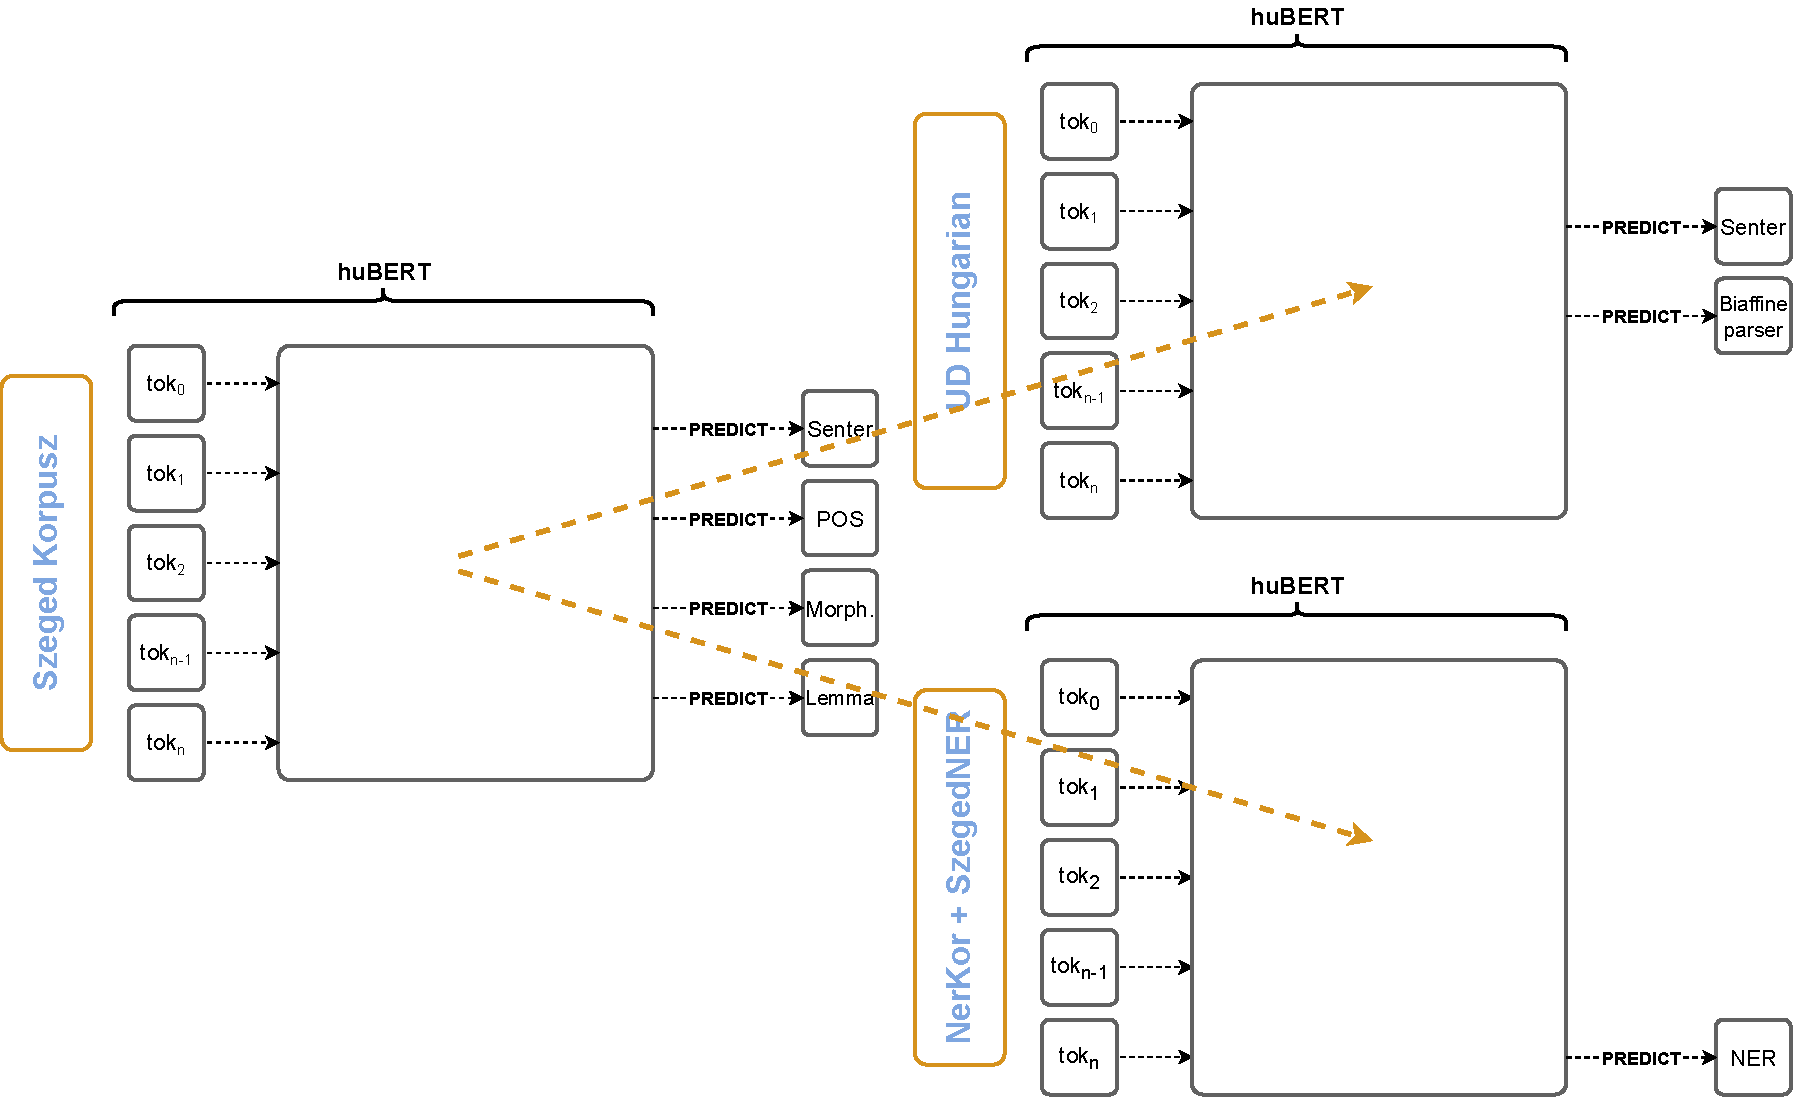
\includegraphics[scale=.40]{Transfer_learning.drawio.pdf}
    \caption{Transfer learning ábrázolása.}
    \label{transfer_learning}
\end{figure}

Ahogy az \ref{transfer_learning}. ábrán is látható, a rendszerünk 3 különálló modellből áll. Az első, Szeged Korpuszon \citep{szc} tanított modell végzi a szófaji egyértelműsítést, lemmatizálást és a morfológiai címkézést. Ezt a modellt lemásoltuk két példányban és továbbtanítottuk az egyiket függőségi elemzésre kiegészítve a mondatra bontás feladattal is, a másikat pedig névelem-felismerésre. Erre azért volt szükség, mert az egyes feladatok tanítására eltérő adatbázisok álltak rendelkezésünkre és így mégis képesek voltunk kihasználni az egyes részfeladatok közötti kapcsolatokat. Függőségi elemzésre a Szeged Korpusznál kisebb, viszont nemzetközileg elterjedt címkekészletet használó magyar Universal Dependencies \citep{nivre2017universal} (UD) korpuszt használtuk. A névelem-felismerőt pedig a NerKor \citep{nerkor} és a SzegedNER \citep{szegedner} összevont korpuszán tanítottuk.

Ez a módszer abban tér el a korábbi \huspacy{} architektúrától, hogy csak 2 modell készült. A Szeged Korpuszon tanult modell tovább volt tanítva az Universal Dependencies korpuszon, amely így már ki volt egészítve a függőségi elemző fejjel. Így nem volt egy külön modell a függőségi elemzésre.
A változtatásra a \trf{} architektúra esetén azért volt szükség, mert a függőségi elemző tanítása közben azt tapasztaltuk, hogy a modell elfelejtette a korábban tanult feladatokat. A lemmatizálás, szófaji egyértelműsítés és morfológiai címkézés feladatok esetén a pontosság lezuhant az első néhány epochban, utána javult minimálisan, de például a morfológiai címkézés esetén 6, a lemmatizálás esetén pedig 27 százalékponttal romlott a pontosság a Szeged Korpuszon tanult modellhez képest.

% wandb biaffine_with_all_transfer keyword: lemma_acc|sents_f|pos_acc|morph_acc

\subsection{Az alapmodell kiegészítései}
\label{biaffine}

A \huspacy{} rendszer által alapértelmezettként használt átmenet-alapú függőségi elemzőt lecseréltük a \spacy{} rendszer által biztosított gráf-alapú, biaffine figyelmi \emph{(attention)} mechanizmussal rendelkező elemzőre \citep{biaffine}. Az eredeti cikkben alkalmazott Bi-LSTM rétegek helyett, ahogy a korábbi feladatokban, itt is \trf{}-alapú architektúrát használtunk.
Az átmenet-alapú rendszerek a függőségi fát osztályozási problémák sorozataként építik fel, amikben lehetőség van két vizsgált szó között él behúzására vagy balról jobbra haladva a vizsgált szavak léptetésére. Ezek a megoldások a mohó, lokális döntéseik miatt rosszul tudnak teljesíteni hosszú mondatok esetén. Ezzel szemben a gráf-alapú elemzők a szavakból, mint csúcsokból felírt teljes gráfban keresik a maximális feszítőfát. 

A névelem-felismerő a függőségi elemzőhöz hasonlóan egy átmenet-alapú megoldást alkalmaz, amit beam search használatával bővítettünk. Ennek lényege, hogy az elemző az egyes lépésekben több korábbi elemzést is figyelembe vesz. A lemmatizálás feladatban a \cite{peti} cikkben használt megoldásokat alkalmaztuk.

A kifejezetten magyar adatokon tanított \hubert{} mellett kísérleteztünk más, többnyelvű modellekkel is, amelyek támogatják a magyar nyelvet is. Az egyik a \bertmulti{} volt, illetve az \roberta{} két különböző méretű változata, az \robertaB{} és az \robertaL{}.

A \hubert{}, a \bertmulti{} és az \robertaB{} mindegyike 12 rétegből áll, amelyek egyenként 768 dimenziós vektorokat használnak. Az előbbi kettő összesen 110 millió paraméterrel rendelkezik, az \robertaB{} pedig 125 millióval. Ezzel szemben az \robertaL{} kétszer annyi réteget és 1024 dimenziós vektorokat használ és összesen 355 millió paraméterrel rendelkezik.

\subsection{Többnyelvű modellek méretcsökkentése}
\label{roberta_size}

A többnyelvű modellek egyik hátránya a nagyobb memóriaigényük, aminek az oka, hogy az eltérő nyelvek szavai miatt sokkal nagyobb szótárra van szükségük. Egynyelvű felhasználás esetén viszont a szótár egy jelentős részére szinte biztosan nincs szükségünk. Ilyenek például a kínai szimbólumok, török betűk, cirill betűk és az azokra épülő szavak, szótöredékek. Ennek kezelésére reguláris kifejezésekkel megszűrtük a két \roberta{} modell szótárát. A jelenlegi szűrés csak magyar nyelvben használt betűket és írásjeleket tartalmazó szótöredékeket hagyta meg.

\section{Eredmények}

Az összes kiértékelés (a névelem-felismerő kivételével) a Hungarian Universal Dependencies Corpus
tesztkészletén \citep{UniDep} készült és a CoNLL 2018 Shared Taskon\footnote{\url{https://universaldependencies.org/conll18/conll18_ud_eval.py}} alkalmazott kiértékelő szkript felhasználásával történt. A nem \trf{}-alapú modellek esetén összehasonlításképpen öt rendszert választottunk. Az első az \emtsv{} \citep{emtsv1, emtsv2, emtsv3, emtsv4, emtsv5}, második az \udpipe{} \citep{udpipe}, a harmadik a \stanza{} \citep{qi2020stanza} és a negyedik a \udify{} \citep{udify}. Ugyanakkor a 2021-ben publikált \huspacyl{} \citep{huspacy} modelljével is összehasonlítottuk.


A \stanza{}\footnote{\url{https://stanfordnlp.github.io/stanza/performance.html}} és \udpipe{}\footnote{\url{https://ufal.mff.cuni.cz/udpipe/1/models}} szerzői már kimérték a rendszerüket az UD teszthalmazon, de ez nem mondható el az \emtsv{}-ről. Itt a rendszert az alapértelmezett konfigurációs beállítások megtartásával lefuttattuk az általunk alkalmazott teszthalmazon. Ugyanakkor fontos kiemelni, hogy az \emtsv{} eredményei olyan szempontból nem számítanak összevethetőnek, hogy nem lett újratanítva az általunk használt adatbázis vágásokkal, hanem csak egyszerű kiértékelés történt. Így a kiértékelés során előfordulhatott átfedés a tanító és a kiértékelő adathalmazok között. A \udify{} kiértékelése során gold adatot használt a tokenizálás és a mondatra bontás feladatokban.

A \trf{}-alapú modellek esetében felhasználtuk az eddigi tapasztalatainkat és további kísérleteket végeztünk néhány egyéb előtanított nyelvi modellel a \huspacy{} mostanra már alapértelmezett konfigurációjával. A következőkben részletesen bemutatjuk az eredményeket, valamint azt is, hogy mely nyelvi modellekkel sikerült elérni őket.

\subsection{Tokenizálás és mondatra bontás}

A mondatra bontás esetén látható, hogy minimálisan, de a \trf{} modellek meghaladják a nem \trf{}-alapú modelleket. Továbbá látható, hogy az \robertaL{}-alapú modell szinte tökéletesen szegmentált, így megelőzve társait.
A tokenizálás semmilyen technikában nem tért el a \huspacy{} cikkben ismertetett módszerektől.

\newlength{\lsz}
\settowidth{\lsz}{Mondatra bontás}
\begin{table}[h]
    % \vspace{2em}
    \begin{center}
        \begin{tabular}{
            l<{\hspace{1em}}
            >{\centering\arraybackslash}m{\lsz}
            >{\centering\arraybackslash}m{\lsz}}
            \toprule
                                      & Token               & Mondatra bontás \\
            \midrule
            \stanza{}                 & \textbf{99,92\%}    & 97,45\%         \\
            \udpipe{}                 & 99,80\%             & 95,90\%         \\
            \emtsv{}                  & 99,77\%             & 98,67\%         \\
            \udify{}                  & --                  & --             \\
            \huspacyl{}               & 99,89\%             & 98,55\%         \\
            \midrule
            \hubert{}                 & 99,89\%             & 99,33\%        \\
            \bertmulti{}              & 99,89\%             & 87,75\%        \\
            \robertaB{}               & 99,89\%             & 99,33\%        \\
            \robertaL{}               & 99,89\%             & \textbf{99,67\%}        \\
            \bottomrule
        \end{tabular}
        \vspace{1em}
        \caption{Mondatra bontás F1-score eredményei az UD teszthalmazán.}
        \label{table:tokens}
    \end{center}
    \vspace{-3em}
\end{table}

\subsection{Morfo-szintaktikai elemzés}

A \ref{table:tagging}. táblázat eredményei alapján elmondható, hogy a \hubert{}-alapú modell kiemelkedően teljesít minden területen. A morfológiai elemzésben sikerült több, mint fél százalékponttal javítani az eddigi legjobb eredményen. A szófaji címkézés esetében szintén sikerült javítani több, mint egy százalékponttal. Ezen felül a lemmatizálás feladatban is legalább 4 százalékponttal javított minden eddigi rendszerhez képest. 

Ugyanakkor összesítve az \robertaL{}-alapú modell ismét majdnem minden más modellt (lemmatizálásnál szinte fej fej mellett van a \hubert{}-alapú modellel) megelőz, morfológiai elemzés esetén is 3 százalékponttal felülmúlja a \hubert{}-alapú modellt.

\newlength{\lm}
\settowidth{\lm}{Morph. acc.}
\begin{table}[h]
    % \vspace{2em}
    \begin{center}
        %\addtolength{\tabcolsep}{-5pt}
        \begin{tabular}{
            l<{\hspace{1em}}
            >{\centering\arraybackslash}m{\lm}
            >{\centering\arraybackslash}m{\lm}
            >{\centering\arraybackslash}m{\lm}
            }
            \toprule
                                     & Lemma pontosság       & PoS pontosság    & Morf. pontosság  \\
            \midrule
            \stanza{}                & 94,19\%               & 96,00\%          & 93,62\%    \\
            \udpipe{}                & 88,50\%               & 90,60\%          & 88,50\%            \\
            \emtsv{}                 & 96,16\%               & 89,19\%          & 89,12\%           \\
            \udify{}                 & 90,19\%               & 96,36\%          & 86,16\%          \\
            \huspacyl{}              & 97,46\%               & 96,89\%          & 93,87\%           \\
            \midrule
            \hubert{}                 & \textbf{98,68\%}    & 97,27\%           & 94,20\%         \\
            \bertmulti{}              & 98,48\%             & 97,11\%           & 91,76\%         \\
            \robertaB{}               & 98,55\%             & 97,73\%           & 96,61\%         \\
            \robertaL{}               & 98,67\%             & \textbf{98,01\%}  & \textbf{97,15\%} \\
            
            \bottomrule
        \end{tabular}
        \vspace{1em}
        \caption{Lemmatizálás, szófaji címkéző (PoS) és morfológiai elemző F1-score eredményei az UD teszthalmazán.}
        \label{table:tagging}
    \end{center}
    \vspace{-2em}
\end{table}

\subsection{Gráf-alapú függőségi elemző}

A \ref{table:parser}. táblázatban látható az átmenet-alapú függőségi elemző, a gráf-alapú függőségi elemző,
illetve a többi rendszer eredményei. Mivel az \emtsv{} nem szolgáltat \ud{} formátumú függőségi
elemzést, így ez a modell nem mérhető ezzel a feladattal.

\newlength{\lmm}
\settowidth{\lmm}{Parser}
\begin{table}[h]
    % \vspace{-1em}
    \begin{center}
    \setlength{\tabcolsep}{10pt}
        \begin{tabular}{
            l<{\hspace{1em}}
            >{\centering\arraybackslash}m{\lmm}
            >{\centering\arraybackslash}m{\lmm}
            }
            \toprule
                                       & UAS                      & LAS       \\
            \midrule
            \stanza{}                  & 84,19\%                  & 79,23\%   \\
            \udpipe{}                  & 72,80\%                  & 67,20\%   \\
            \udify{}                   & 89,69\%                  & 84,88\%          \\
            \huspacyl{}                & 82,53\%                  & 75,56\%   \\
            \midrule
            \hubert{} - átmenet-alapú  & 89,95\%                  & 83,94\%  \\
            \hubert{} - gráf-alapú     & \textbf{91,57\%}         & \textbf{87,58\%}  \\
            \midrule
            \bertmulti{} - gráf-alapú              & 85,92\%                 & 81,93\%           \\
            \robertaB{} - gráf-alapú               & 89,47\%                 & 86,02\%           \\
            \robertaL{} - gráf-alapú               & 90,38\%                 & 86,88\%          \\
            \bottomrule
        \end{tabular}
        \vspace{1em}
        \caption{Átmenet-alapú és gráf-alapú függőségi elemzés összehasonlítása a meglévő rendszerekkel, illetve a magyar nyelvre elérhető \trf{}-alapú nyelvi modellek kiértékelése.}
        \label{table:parser}
    \end{center}
    \vspace{-3em}
\end{table}

A meglévő rendszerek és a \huspacyl{} modellje is alulmarad a \hubert{} átmenet-alapú modellel szemben, mind az UAS és a LAS tekintetében is. Az átmenet-alapú függőségi elemzővel rendelkező \hubert{}-alapú modell viszont alulmarad a már tárgyalt gráf-alapú megoldással szemben. Ezért ezt alkalmaztuk is a továbbiakban, illetve a többi \trf{}-alapú modellnél is ezt használtuk alapértelmezett elemzőként függőségi elemző esetén.

Viszont ebben a feladatban az \robertaL{} pontatlanabb a \hubert{} gráf-alapú modellel szemben. Ez az egyetlen olyan komponens, ahol a \hubert{}-alapú modell sokkal jobban teljesít az \robertaL{}-alapú modellnél.

\subsection{Névelem-felismerés}

Mivel az UD korpusz nem tartalmaz névelemeket, ezért erre a célra a NerKor \citep{nerkor} és a SzegedNER \citep{szegedner} korpuszt használtuk. Mivel az \udpipe{}-ban nincs névelem-felismerő, így azt nem lehetett bevonni a vizsgálatba. Három korábbi névelem-felismerőt is bevettünk az összehasonlításba. Az egyik a \cite{szarvas-ner}, amely döntési fákat használ. A második a \cite{simon-ner}, amely egy lineáris modellt használ és rejtett Markov modelleket kombináló statisztikai címkézővel rendelkezik. A harmadik, újabb rendszer pedig az \embert{}, amely egy \trf{}-alapú NER modell. A \stanza{} esetén viszont fontos kiemelni, hogy újra lett tanítva az általunk használt adatbázisokkal \citep{nerkoreval}. 

\newlength{\lnersz}
\settowidth{\lnersz}{SzegedNer}
\begin{table}[h]
    \begin{center}
        \begin{tabular}{
            l<{\hspace{1em}}
            >{\centering\arraybackslash}m{\lnersz}
            >{\centering\arraybackslash}m{\lnersz}
            >{\centering\arraybackslash}m{\lnersz}
            }
            \toprule
                                    & SzegedNER & NerKor  & Kombinált        \\
            \midrule
            \cite{simon-ner}        & 95,06\%   & --      & --               \\
            \cite{szarvas-ner}      & 94,77\%\  & --      & --               \\
            \embert{}               & 97,40\%   & 92,09\% & \textbf{92,99\%} \\
            \stanza{}               & 91,78\%   & 80,53\% & 83,75\%          \\
            \huspacyl{}             & 95,31\%   & 80,75\% & 85,73\%          \\
            \midrule
            \hubert{}                     & 97,01\%    & 88,27\% & 90,26\%   \\
            \hubert{} + beam search       & 97,37\%    & 89,13\% & 91,27\%   \\
            \midrule
            \bertmulti{} + beam search              & --    & --   & 89,07\%         \\
            \robertaB{} + beam search               & --    & --   & 90,94\%         \\
            \robertaL{} + beam search               & --    & --   & \underline{91,86\%}   \\
            \bottomrule
        \end{tabular}
        \vspace{1em}
        \caption{F1-scoreon mért névelem-felismerés összehasonlítása a SzegedNER, a NerKor és a kombinált teszthalmazon is.}
        \label{table:ner_cmp}
    \end{center}
    \hspace*{.1\linewidth}
    \vspace{-4em}
\end{table}

A NerKor adatbázis esetében a szerzők által meghatározott tanító-validáló-teszt halmazokra
bontást alkalmaztuk. A SzegedNER esetében pedig, az összehasonlítás érdekében, a \cite{szarvas-ner} cikk által meghatározott vágás lett felhasználva. 

A meglévő rendszerek, az \embert{} kivételével, alulmaradnak a \huspacyl{} modellel és a \hubert{}-alapú modellel szemben. Viszont a \hubert{}-alapú + beam search modell jobb eredményt ért el, mint ahol nem volt alkalmazva a beam search, ahogy a \ref{table:ner_cmp}. táblázatban is látható. A konklúzió tehát, hogy jobb a beam search, ezért a többi \trf{}-alapú modellnél is ezt használtuk alapértelmezett módszerként.

Így, mivel bevettük a vizsgálatba a régebbi rendszereket, ezért külön korpuszokra is le lettek mérve a modellek. Az \embert{}-tel való összehasonlítás során a SzegedNER korpusz esetében szinte fej fej mellett van a két modell (\embert{} és a beam search \hubert{}-alapú modell), de a NerKor esetében kicsit alulmarad a \hubert{}-alapú modell. A kombinált korpuszon is jobb az \embert{}, mert a 12 réteg feletti Viterbi-algoritmus garantálja a jósolt címkeszekvencia konzisztenciáját. Ezen felül, ha megnézzük az összes \trf{}-alapú modellt és az \embert{} eredményeit, kijelenthető, hogy az utóbbi továbbra is a leghatékonyabb.

\subsection{\roberta{}-hu modell méretcsökkentése}

Ahogyan a \ref{roberta_size}. fejezetben említettük, az \roberta{} modellek méretét, ha sikerülne csökkenteni megtartva a teljesítményét, akkor elérhető lenne egy rendkívül pontos modell jelentősen kevesebb memóriaigénnyel.

Az első fázisban reguláris kifejezések segítségével szűrtük ki azokat a tokeneket, amelyek nem fellelhetőek a magyar és az angol nyelvben. Így például a kínai szimbólumokat, török betűket, cirill betűket tartalmazó részszavakat és karaktereket kivettük. Ugyanakkor az Embedding layerből is eltávolítottuk a hozzátartozó vektorokat, így a paraméterszáma is csökkent a modellnek.

\newlength{\lroberta}
\settowidth{\lroberta}{98,56\%aa}
\newlength{\lrobertalem}
\settowidth{\lrobertalem}{Lemmatizálás}
\begin{table}[h]
    % \vspace{-2em}
    \begin{center}
    \setlength{\tabcolsep}{1pt}
        \begin{tabular}
            {
            l<{\hspace{1em}}
            >{\centering\arraybackslash}m{\lroberta}
            >{\centering\arraybackslash}m{\lroberta}
            >{\centering\arraybackslash}m{\lroberta}
            >{\centering\arraybackslash}m{\lroberta}
            >{\centering\arraybackslash}m{\lrobertalem}
            }
            \toprule
                            & Token                              & Mondatra bontás                & PoS                 & Morf.               & Lemma          \\
            \midrule
            \robertaB{}     & \textbf{\multirow{2}{*}{99,89\% }} & \underline{99,33\%}  & \underline{97,73\%} & \underline{96,61\%} & \underline{98,55\%} \\
            \robertahub{}   &                                    & 98,56\%              & 97,60\%             & 96,27\%             & 98,42\%             \\
            \midrule
            \robertaL{}     & \textbf{\multirow{2}{*}{99,89\% }} & \textbf{99,67\%}     & \textbf{98,01\%}    & \textbf{97,15\%}    & \textbf{98,67\%}    \\
            \robertahul{}   &                                    & 97,24\%              & 97,46\%             & 95,84\%             & 98,11\%             \\
            \bottomrule
        \end{tabular}
        \vspace{1em}
        \caption{Módosított \roberta{} modellek F1-score eredményei az UD korpuszon. (Az aláhúzás az aktuális résztáblázatban a legjobb eredmény, a félkövérített pedig az adott egész táblázatban a legjobb eredmény.)}
        \label{table:roberta}
    \end{center}
    % \hspace*{-4\linewidth}
    \vspace{-3em}
\end{table}

\newlength{\lrobertaa}
\settowidth{\lrobertaa}{XLMRoBERTa2}
\begin{table}[h]
    % \vspace{-2em}
    \begin{center}
    % \setlength{\tabcolsep}{10pt}
        \begin{tabular}
            {
            l<{\hspace{1em}}
            >{\centering\arraybackslash}m{\lrobertaa}
            >{\centering\arraybackslash}m{\lrobertaa}
            >{\centering\arraybackslash}m{\lrobertaa}
            }
            \toprule
                            & UAS                 & LAS                 & NER        \\
            \midrule
            \robertaB{}     & \underline{89,47\%} & \underline{86,02\%} & \underline{90,94\%}  \\
            \robertahub{}   & 89,21\%             & 85,54\%             & 89,89\%           \\
            \midrule
            \robertaL{}     & \textbf{90,38\%}    & \textbf{86,88\%}    & \textbf{91,86\%}  \\
            \robertahul{}   & 89,40\%             & 85,46\%             & 90,44\%           \\
            \bottomrule
        \end{tabular}
        \vspace{1em}
        \caption{Módosított \roberta{} modellek UAS és LAS eredményei az UD korpuszon, a NER pedig a kombinált NER adatbázison lett mérve, amely F1-scoret mutatnak.}
        \label{table:roberta2}
    \end{center}
    % \hspace*{-4\linewidth}
    \vspace{-3em}
\end{table}

Ahogy a \ref{table:roberta}. és a \ref{table:roberta2}. táblázatokban is észrevehető, a méretoptimalizált modellekkel hozzávetőlegesen sikerült tartani a teljesítményt. Jelenlegi kísérletek is hasznos eredményeknek számítanak, ugyanis az \robertahub{} esetén például sikerült a \textbf{felére csökkenteni} a méretet és az \robertahul{} modell pedig megközelítőleg \textbf{kétharmada az eredetinek}. Ezt a következő fejezetben jobban kifejtjük és összehasonlítjuk. Konklúzió, hogy a jelenlegi módszer segítségével képesek vagyunk csökkenteni a \roberta{} modell méretét minimális pontosságvesztéssel. Annak érdekében, hogy valóban hasznos legyen ez a modell és megtartsa a pontosságot, szükség lenne egy olyan heurisztikára, amely képes lenne ezt a feladatot ellátni. Jövőbeli tervünk, hogy az eldobandó szótöredékek halmazát statisztikai alapon válasszuk ki. Ehhez szeretnénk felhasználni a WebCorpus 2.0-át \citep{Nemeskey:2020} és csak az abban előforduló leggyakoribb szótöredékeket megtartani, amivel a terveink szerint tovább csökkenthetnénk a szótár méretét és megtarthatnánk olyan speciális karaktereket is, amiket a kézi szabályokkal nem fedtünk le. A jelenlegi script elérhető publikus módon a GitHubon\footnote{\url{https://github.com/huspacy/huspacy-resources/blob/master/scripts/XLM-RoBERTa_size_reduction/XLM-RoBERTa_size_reduction.ipynb}}, ami lehetővé teszi egy új specifikus nyelvi modell készítését bármely nyelvre.


\subsection{Memóriahasználat}

A \trf{} architektúrák esetén fontosak az erőforrásigények, ezért ebben a fejezetben mélyebben megvizsgáljuk a futásidőket és a memóriaigényeket az összes eddigi modell szemszögéből. Az \udpipe{}, \emtsv{} és az \udify{} rendszerek nem támogatják a névelem-felismerést, így ezeket a modelleket a névelem-felismerő nélkül mértük. A mérések az UD teszthalmazán készültek.

\newlength{\lper}
\settowidth{\lper}{Throughput tok}
\begin{table}[h]
    \begin{center}
    % \setlength{\tabcolsep}{1pt}
        \begin{tabular}{
            l<{\hspace{1em}}
            >{\centering\arraybackslash}m{\lper}
            >{\centering\arraybackslash}m{\lper}
            >{\centering\arraybackslash}m{\lper}
            }
            \toprule
                                      & Gyorsaság (token/mp) CPU & Gyorsaság (token/mp) GPU & Memóriahasználat (GB) \\
            \midrule
            \stanza{}                 & 30         & 395        & 5,3  \\
            \udpipe{}                 & 3175       & --         & 1,3  \\
            \emtsv{}                  & 113        & --         & 3,9  \\
            \udify{}                  & 129        & 475        & 3,2  \\
            \huspacyl{}               & 728        & 4685       & 3,2  \\
            \midrule
            \hubert{}                 & 176        & 2605        & 4,8  \\
            \bertmulti{}              & 138        & 2631        & 7,0  \\
            \robertaB{}               & 151        & 2847        & 11,2 \\
            \robertahub{}             & 166        & 3265        & 6,2  \\
            \robertaL{}               & 50         & 2353        & 18,9 \\
            \robertahul{}             & 59         & 2390        & 14,6 \\
            \bottomrule
        \end{tabular}
        \vspace{1em}
        \caption{A CPU-n (AMD EPYC 7F72) és GPU-n (NVIDIA A100 40 GB) összehasonlított rendszerek gyorsasága (token/másodpercben mérve) és a maximális memóriahasználatuk.}
        \label{table:performance}
    \end{center}
    \vspace{-3em}
\end{table}

Először nézzünk meg a CPU-s oszlopot. A \ref{table:performance}. táblázatban jól látható, hogy a \trf{} modellek a többi rendszerekhez képest több erőforrást igényelnek. Viszont kivételt képez például az \emtsv{} gyorsasága a \hubert{}-alapú modellhez képest. A \stanza{} szintén lassabb, memóriaigények tekintetében pedig egy skálán mozognak. Az \udpipe{}
ellenben mind a két esetben jól teljesített a futásidő és memóriaigények tekintetében, ugyanakkor ez a rendszer minden elemző esetén alulmarad hatékonyságban a többi rendszerhez képest. A többi \trf{} modell több paraméterrel rendelkezik, ezért és a többnyelvűség miatt is több erőforrást igényelnek. 

Megfigyelhető az is, hogy a \hubert{}-alapú modell memóriahasználatban a \huspacyl{} modelljéhez képest nem mutat jelentős eltérést. Ellenben az \roberta{} modellekre ez már nem teljesen igaz. Ahogyan szó volt a \ref{transfer_learn}. fejezetben a modellek összetételéről, itt nyilvánul meg a három \trf{} modell mérete és az, hogy a többnyelvű modellek sokkal több memóriát igényelnek már önmagukban is.

A méretoptimalizált és az eredeti modellek között a futásidő azért nem változott drasztikusan, mert tulajdonképpen mind a két esetben ugyanazok a neuronok feleltek a futásidőért. Más szóval, a modell csak azon neuronokat használta fel a predikáláshoz, amelyekre a magyar nyelvhez szükség van. Az, hogy el lettek távolítva azok a részek, amelyeket a modell egyébként sem használt, nem befolyásolta a futásidőt.

\section{Összegzés}

Elkészítettünk a \huspacy{}-hez\footnote{\url{https://github.com/huspacy/huspacy/tree/develop}} egy \hubert{}-alapú %\trf{} 
modellt\footnote{\url{https://huggingface.co/huspacy/hu_core_news_trf}}, ami minden
hagyományos nyelvi elemzőt tartalmaz, vagyis tokenizálót, mondatra bontót, lemmatizálót, szófaji és morfológiai egyértelműsítőt, függőségi elemzőt, illetve ezeken felül névelem-felismerőt is és ezen eredmények teljes mértékben reprodukálhatóak. 

Összességében a \trf{}-alapú modellek minden feladatban jobb eredményt érnek el a korábbi megoldásoknál. Ezek közül is a legtöbb feladatban a \robertaL{} teljesített a legjobban, csupán a függőségi elemzés részfeladaton múlta felül a \hubert{}-alapú modell. Az alacsonyabb memóriaigényének és gyorsabb futásának köszönhetően a \hubert{} sok esetben jó választás lehet, de, ha a pontosságon van a hangsúly, a \robertaL{} felhasználásával érhetjük el a legjobb eredményt.
Viszont a state-of-the-art eredmények ellenére is hátrányt jelenthet bizonyos végalkalmazásokban a nagyobb erőforrásigényük, például időérzékeny alkalmazásokban, illetve, ha korlátozott erőforrásokkal rendelkezünk. Ezekben a szituációkban megfelelő döntés lehet a \huspacyl{} modell használata.

A függőségi elemzés és a névelem-felismerés problémákra több algoritmust is kipróbáltunk és a legmegfelelőbbet alkalmaztuk. Az eredmények alapján, a \hubert{}-alapú modell a függőségi elemző esetén hatalmas javulást mutat az elődeihez képest, így sikerült egy state-of-the-art eredményt elérni. Továbbá a morfológiai elemzés esetén is az \robertaL{}-alapú modell képest volt 4 százalékponttal javulni az eddigi legjobb eredményhez képest.

Az elkészült modellek bárki számára szabadon igénybe vehetők a nyílt forráskódú \huspacy{} részeként.

\section*{Köszönetnyilvánítás}

A kutatás az Európai Unió támogatásával valósult meg, az
RRF-2.3.1-21-2022-00004 azonosítójú, Mesterséges Intelligencia Nemzeti Laboratórium projekt keretében. Továbbá szeretnénk megköszönni Berend Gábor segítségét a nyelvi modellek méretcsökkentésével kapcsolatban.

\renewcommand\bibname{Hivatkoz\'asok}

\bibliographystyle{splncsnat}
\bibliography{main}

\end{document}